% =============================================================
% Chapter 6: Project Design
% =============================================================

\newpage
\vspace*{\fill}
\begin{center}
\textbf{\Huge{Chapter 6}}\\
\vspace{5mm}
\textbf{\Huge{Project Design}}
\end{center}
\vspace*{\fill}
\newpage

\titleformat{\chapter}[block]{\normalfont}{}{0pt}{}
\titlespacing{\chapter}{0pt}{-2em}{0pt}
\chapter[Project Design]{}
\titleformat{\chapter}[display]{\vspace{1cm}\normalfont\Large\bfseries\centering}{\chaptertitlename\ \thechapter}{20pt}{\vspace{0pt}}
\titlespacing*{\chapter}{0pt}{-50pt}{20pt}

\section{Data Flow Diagram}
\vspace{1cm}

\subsection{Level 0 DFD}

\sloppy
The Level 0 Data Flow Diagram (DFD) delineates the boundary interactions of the AyurSpace System. The central process (0) interfaces outward primarily to three entity bodies: The Mobile User End Device, the Firebase Cloud, and the external intelligence nodes (Plant.id and Google Gemini). User inputs credentials, images, and text queries. The system relays processed image arrays and text prompts out, securing taxonomic confidence arrays and Ayurvedic response text back, whilst syncing overall profiles securely with the Firebase cloud.
\fussy

\vspace{1cm}
\renewcommand{\thefigure}{6.1.1}
\begin{figure}[h]
\begin{mdframed}
     \centering
    
\includegraphics[width=0.7\linewidth,keepaspectratio]{placeholder_dfd0.png}
\end{mdframed}
 \caption{Level 0 DFD}
\end{figure}
\newpage

\subsection{Level 1 DFD}
The Level 1 Data Flow Diagram breaks apart process 0 into dedicated internal components: Authentication Management (1.0), Image Processing \& Vision (2.0), Ayurvedic Reasoning Engine (3.0), and Health Profiling (4.0). Interaction between data stores (D1: User Profiles, D2: Scan History) is clear. Raw images get translated via external APIs within 2.0, the context flows into 3.0 alongside Gemini LLMs, and Profiling calculations merge into reasoning to yield tailored health output.

\vspace{0.5cm}
\renewcommand{\thefigure}{6.1.2}
\begin{figure}[!htpb]
\begin{mdframed}
    \centering
    
\includegraphics[width=\linewidth,height=0.8\textheight,keepaspectratio]{placeholder_dfd1.png}
\end{mdframed}
    \caption{Level 1 DFD}
\end{figure}

\newpage

\section{Flow Chart}
The Flowchart maps out the navigation behavior within the app. Upon start, it verifies Auth. From the Home Dashboard, users branch their activities into Scanning (where invalid taxonomy trips alerts), Chatting (invoking Gemini query handling context rules), or executing assessments (which re-run scoring algorithms upon user completion). The design demonstrates systematic state transitions within the multi-faceted toolkit.

\renewcommand{\thefigure}{6.2}
\begin{figure}[!htpb]
\begin{mdframed}
    \centering
   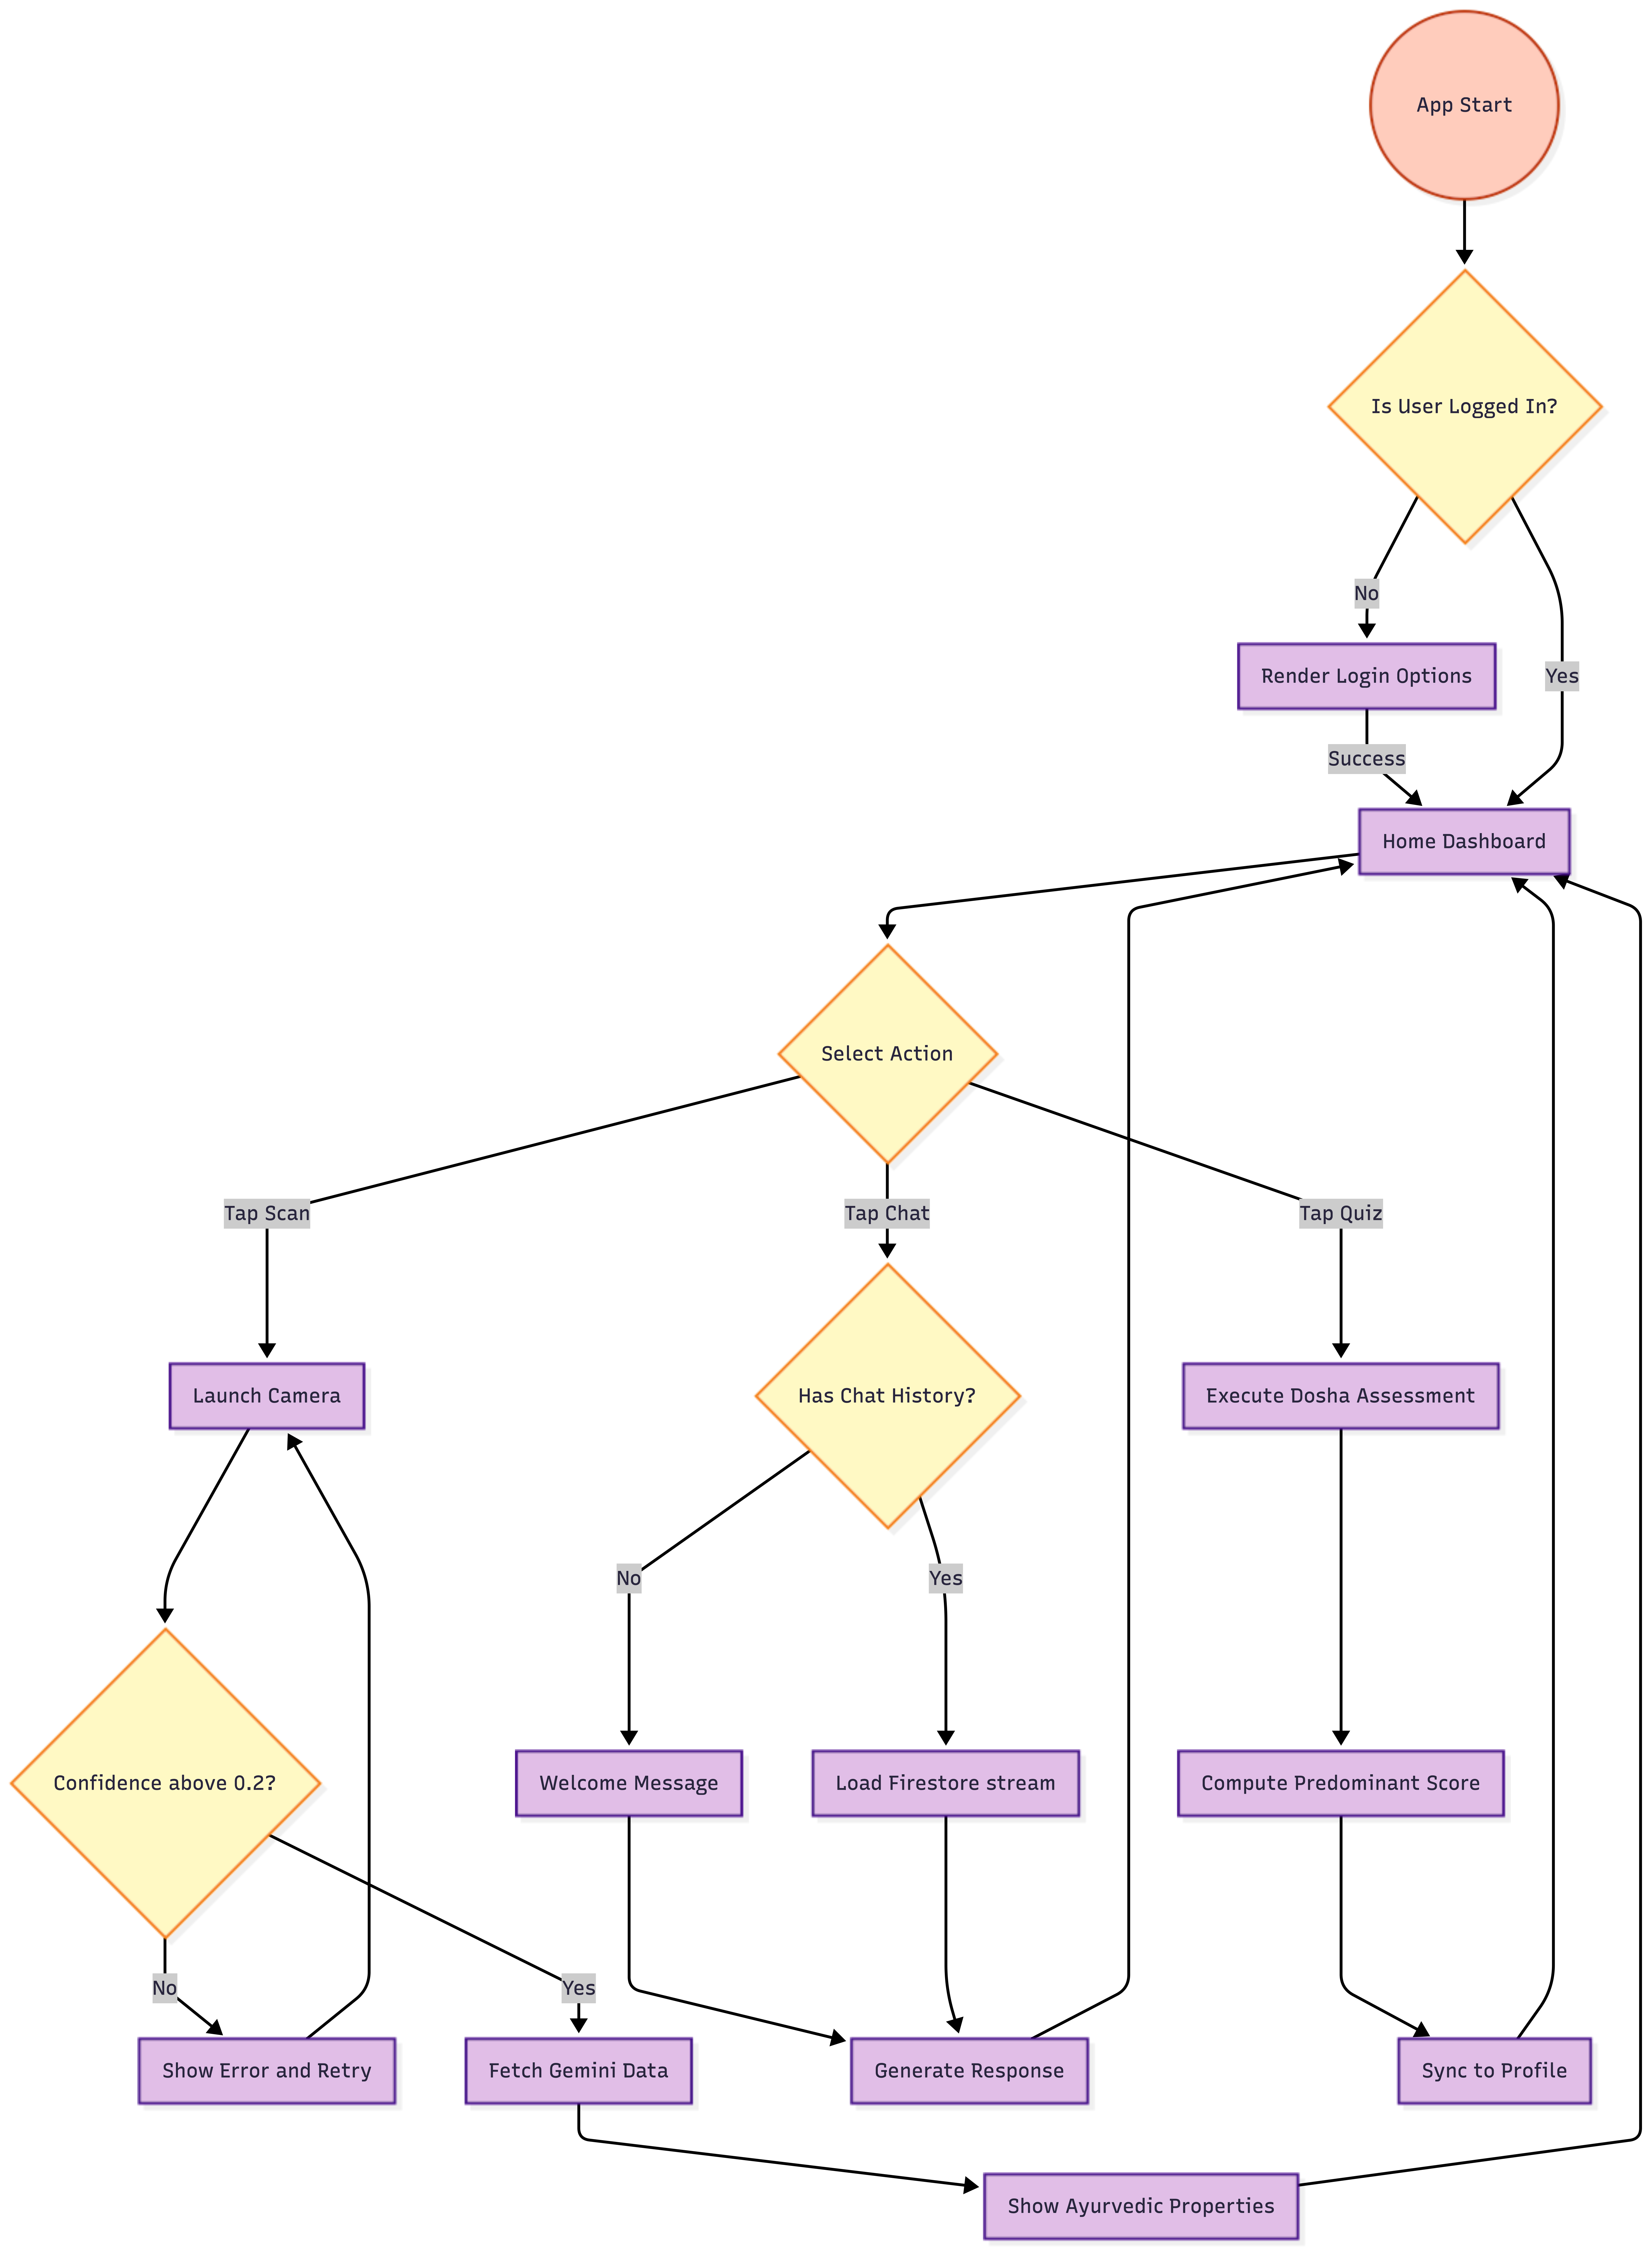
\includegraphics[width=\linewidth,height=0.7\textheight]{placeholder_flowchart.png}
\end{mdframed}
\caption{Flow Chart}
\end{figure}
